\documentclass[11pt,a4paper]{article}
\usepackage[a4paper,left=2.0cm,right=2.0cm,top=1.55cm,bottom=1.55cm]{geometry}
\usepackage[T1]{fontenc}
\usepackage{lmodern}
\usepackage{graphicx}
\usepackage{xcolor}
\usepackage{array}
\usepackage{tabularx}
\usepackage{ragged2e}
\usepackage{enumitem}
\usepackage{fancyhdr}
\usepackage{tikz}
\usetikzlibrary{arrows.meta,positioning}
\usepackage{setspace}


\definecolor{TitleBlue}{RGB}{61,103,154}


\setlength{\parindent}{0pt}
\setlength{\parskip}{0pt}
\renewcommand{\arraystretch}{1.0}

\newcommand{\blueheading}[1]{%
    {\sffamily\color{TitleBlue}\fontsize{15}{18}\selectfont #1}%
}

\newcommand{\bluebigheading}[1]{%
    {\sffamily\bfseries\color{TitleBlue}\fontsize{16}{19}\selectfont #1}%
}

\newcommand{\answerbox}[1]{%
    \vspace{2pt}%
    \noindent
    \fbox{%
        \begin{minipage}[t]{\dimexpr\textwidth-2\fboxsep-2\fboxrule\relax}
            \vspace{2mm}
            \itshape #1\par
            \vspace{2mm}
        \end{minipage}%
    }%
}

\pagestyle{fancy}
\fancyhf{}
\renewcommand{\headrulewidth}{0pt}
\renewcommand{\footrulewidth}{0pt}

\fancyhead[L]{%
    \sffamily\bfseries\itshape\fontsize{10.5}{12}\selectfont
    CSE -- DSCPP-III-2026-T226
}
\fancyhead[R]{%
    \sffamily\bfseries\fontsize{10.5}{12}\selectfont
    INTELLIGENT TRAFFIC OPTIMIZATION SYSTEM
}
\fancyfoot[R]{%
    \itshape\fontsize{10}{12}\selectfont
    Page \thepage
}
\setlength{\headheight}{14pt}
\setlength{\headsep}{23pt}
\setlength{\footskip}{24pt}

\begin{document}

\vspace*{4mm}

\bluebigheading{PROJECT AND TEAM INFORMATION}

\vspace{10mm}

\blueheading{Project Title}

\vspace{2mm}

\answerbox{Intelligent Traffic Optimization System}

\vspace{10mm}

\blueheading{Student / Team Information}

\vspace{2mm}

\noindent
\begin{tabularx}{\textwidth}{|>{\RaggedRight\arraybackslash}p{0.38\textwidth}|>{\RaggedRight\arraybackslash}X|}
\hline
\begin{minipage}[t]{\linewidth}
\vspace{1.5mm}
\textit{Team ID:}
\vspace{1.5mm}
\end{minipage}
&
\begin{minipage}[t]{\linewidth}
\vspace{1.5mm}
\textit{DSCPP-III-2026-T226}
\vspace{1.5mm}
\end{minipage}
\\
\hline
\begin{minipage}[t]{\linewidth}
\vspace{2mm}
\textbf{Team member 1 (Team Lead)}\\[-1mm]
\textit{(Last Name, name: student ID: email, picture):}
\vspace{2mm}
\end{minipage}
&
\begin{minipage}[t]{\linewidth}
\vspace{2mm}
\textit{Akshita -- 2510012193}\\
\textit{akshitachourdhary8923@gmail.com}

\vspace{2mm}
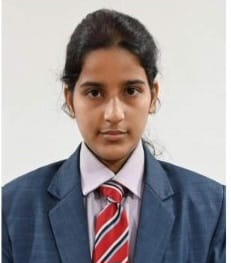
\includegraphics[width=3.0cm,height=1.5cm,keepaspectratio]{member1.png}
\vspace{2mm}
\end{minipage}
\\
\hline
\begin{minipage}[t]{\linewidth}
\vspace{2mm}
\textbf{Team member 2}\\[-1mm]
\textit{(Last Name, name: student ID: email, picture):}
\vspace{2mm}
\end{minipage}
&
\begin{minipage}[t]{\linewidth}
\vspace{2mm}
\textit{Singh, Vaani -- 2510360148}\\
\textit{vaanisingh56@gmail.com}

\vspace{2mm}
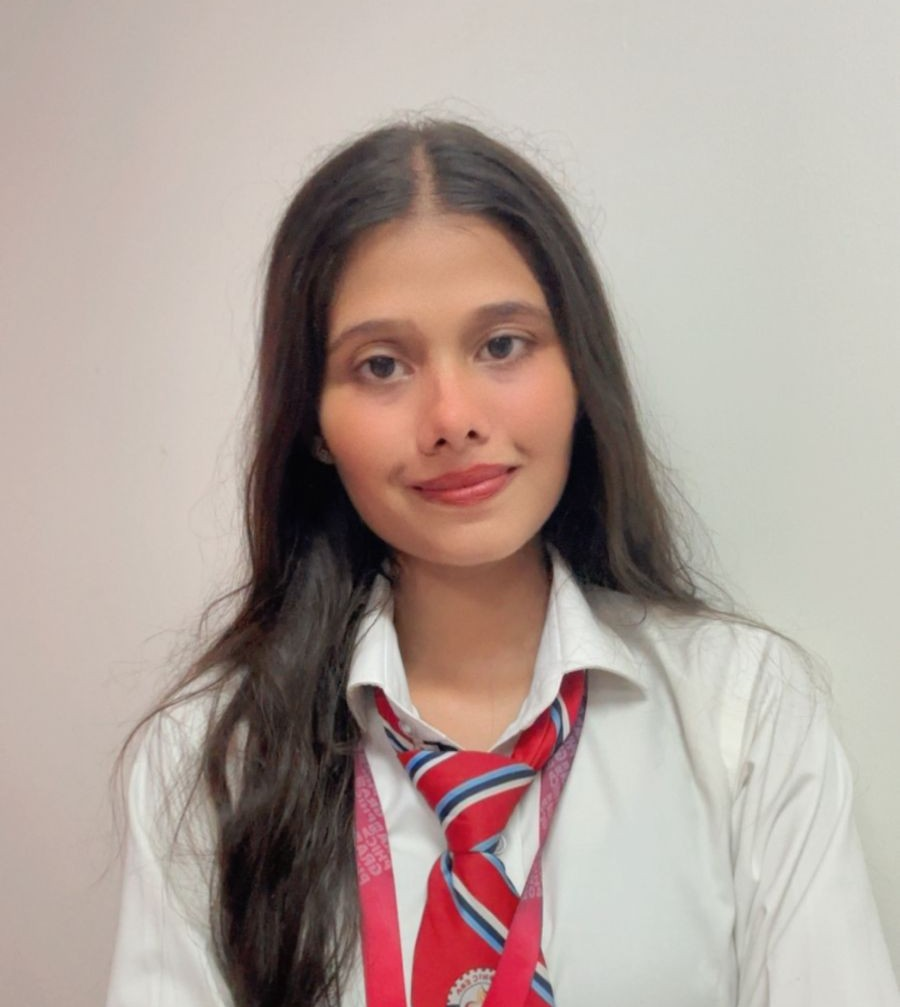
\includegraphics[width=3.0cm,height=1.5cm,keepaspectratio]{member2.png}
\vspace{2mm}
\end{minipage}
\\
\hline
\begin{minipage}[t]{\linewidth}
\vspace{2mm}
\textbf{Team member 3}\\[-1mm]
\textit{(Last Name, name: student ID: email, picture):}
\vspace{2mm}
\end{minipage}
&
\begin{minipage}[t]{\linewidth}
\vspace{2mm}
\textit{Yadav, Panshu -- 2510350036}\\
\textit{Panshu.yadav22@gmail.com}

\vspace{2mm}
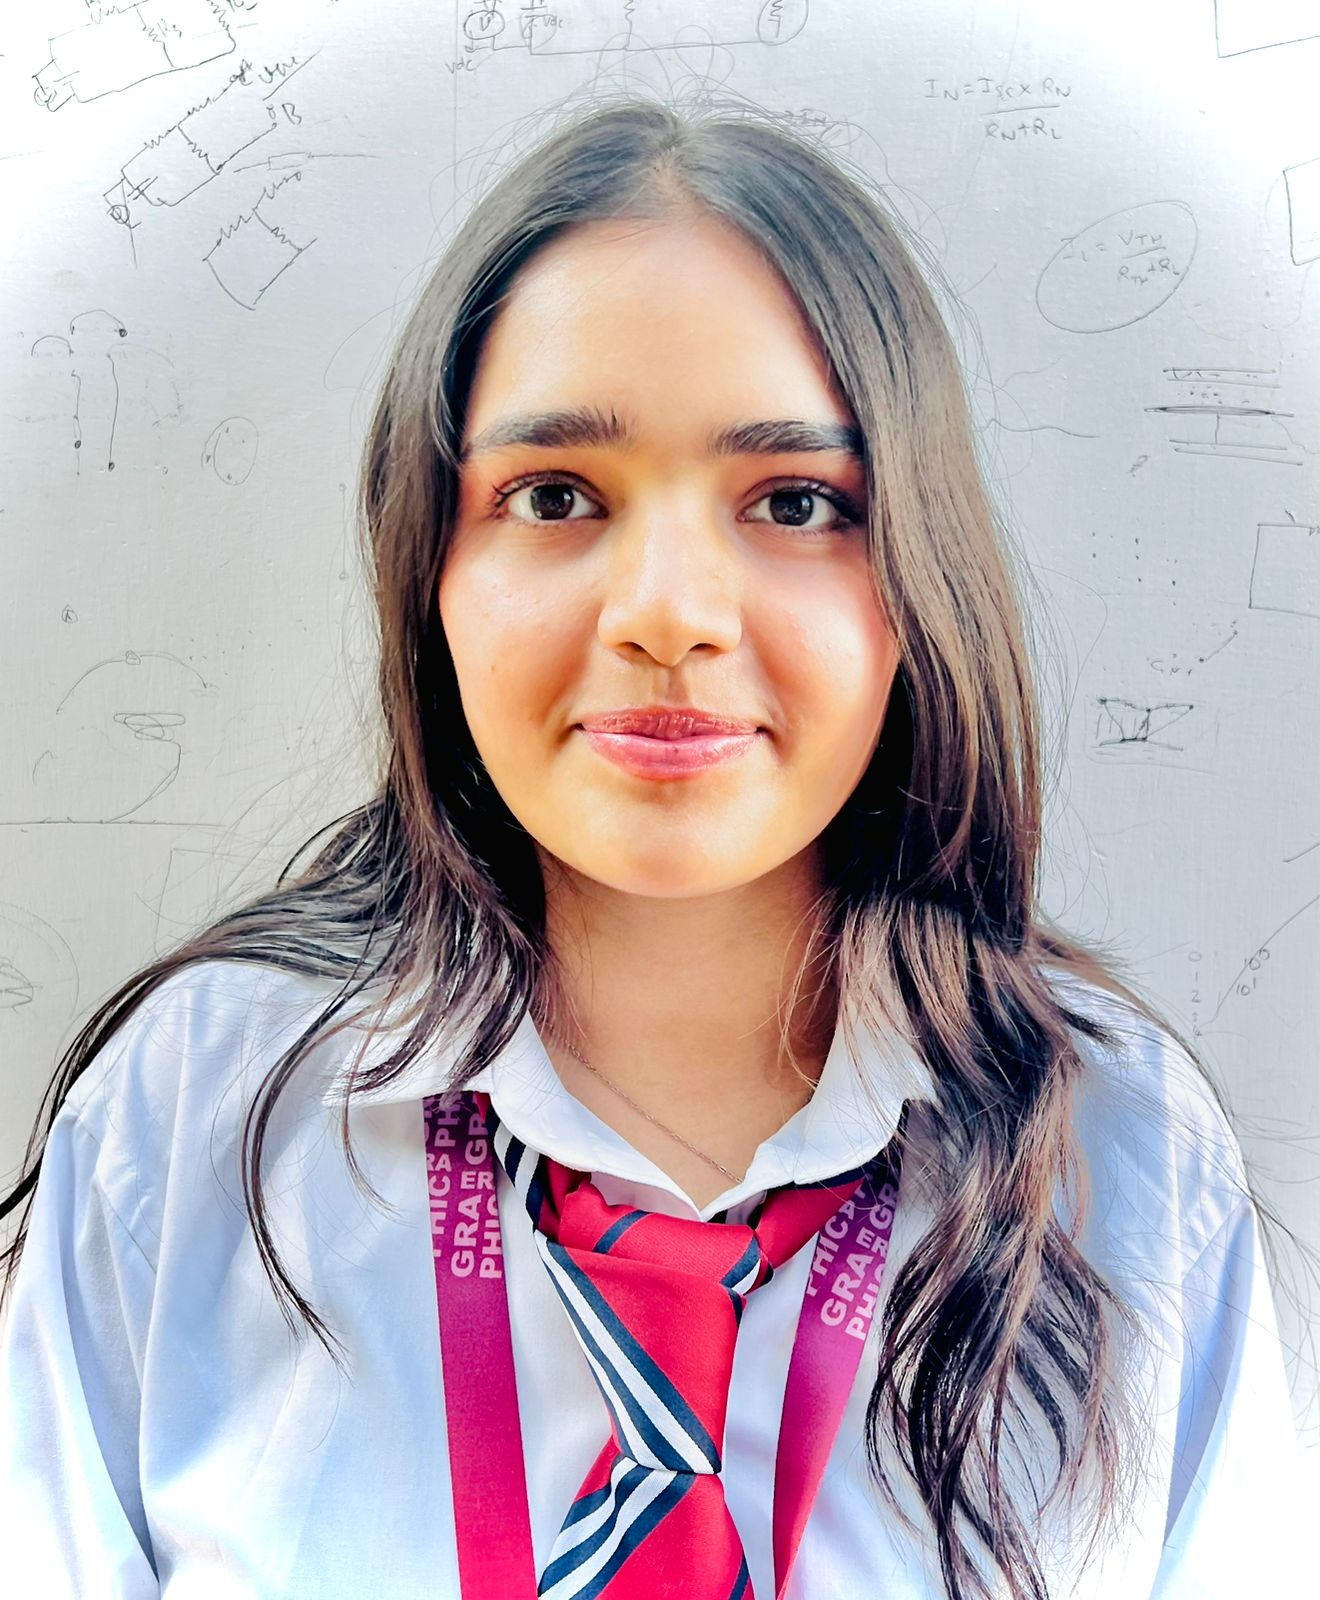
\includegraphics[width=3.0cm,height=1.5cm,keepaspectratio]{member3.png}
\vspace{2mm}
\end{minipage}
\\
\hline
\end{tabularx}

\newpage

\bluebigheading{PROPOSAL DESCRIPTION }

\vspace{6mm}

\blueheading{Motivation }

\vspace{2mm}

\answerbox{The majority of urban intersections currently feature pre-set timing schedules for controlling traffic signals. As such, drivers often find themselves waiting at a red light for no traffic to pass on the crossroad while wasting fuel or causing congestion on the roadways. Space is a premium in most urban areas, and it cannot be expanded to meet the growing demand; therefore, transportation engineers should explore opportunities to optimize the usage of the available road space. The proposed project aims to develop a dynamic signal control simulation that can accurately apportion traffic intervals to roads based on the volume of traffic and provide priority access to emergency vehicles.}

\vspace{6mm}

\blueheading{State of the Art / Current solution }

\vspace{2mm}

\answerbox{The majority of current traffic signals are managed by simple pre-set timing schedules that do not account for prevailing traffic conditions. A few modern traffic lights employ simple sensor plates or timers to create slightly more optimized solutions that operate on a per-intersection level. More advanced solutions utilize high-resolution cameras and artificial intelligence to monitor traffic in real-time and adjust signal timings accordingly. However, such solutions are extremely expensive to install and maintain and can only be afforded in advanced countries. As such, the majority of traffic lights continue to utilize primitive timing schedules that do not account for traffic conditions, causing preventable bottlenecks.}

\vspace{6mm}

\blueheading{Project Goals and Milestones }

\vspace{2mm}

\answerbox{\textbf{General Goals:} Develop an intersection control simulation that tracks vehicle volume per lane, calculates road congestion on the fly, dynamically adjusts green intervals, and provides priority clearance for emergency vehicles.

\vspace{2mm}
\textbf{Milestones:}
\begin{enumerate}[leftmargin=5mm, itemsep=0.3mm, parsep=0pt, topsep=1mm]
    \item Milestone 1: Complete the input module that simulates arrival rates and counts vehicles per lane.
    \item Milestone 2: Implement logic to calculate real-time traffic volume and density percentages for each road.
    \item Milestone 3: Construct core decision algorithms utilizing Queues, Priority Queues, and Graphs.
    \item Milestone 4: Design and implement the simulation engine to manage intersection cycle flow.
    \item Milestone 5: Integrate all software components in C++ to build a unified simulation testbed.
    \item Milestone 6: Benchmark dynamic timing performance against standard pre-set cycles.
\end{enumerate}}

\newpage

\blueheading{Project Approach }

\vspace{2mm}

\answerbox{The project will be implemented in C++ using an object-oriented paradigm centered around \textit{TrafficSignal}, \textit{Road}, and \textit{Vehicle} classes. Key algorithms are built directly upon classical data structures:
\begin{itemize}[leftmargin=5mm, itemsep=0.4mm, parsep=0pt, topsep=1.5mm]
    \item \textbf{Queue (FIFO):} Holds waiting vehicles sequentially per lane and releases them in their order of arrival when signaled green.
    \item \textbf{Priority Queue:} Ranks incoming road approaches based on live vehicle density and emergency flags to decide which road gets the next green phase.
    \item \textbf{Graph Structure:} Models the interconnected road network topology and intersection junctions as vertices and directed edges.
    \item \textbf{Stack:} Logs signal transition history chronologically, enabling state review and event tracing.
    \item \textbf{Linked List:} Dynamically manages in-memory records of active vehicles entering and departing the intersection.
    \item \textbf{Arrays \& Control Loops:} Tracks vehicle counts per approach and drives the core simulation execution loop.
\end{itemize}}

\vspace{6mm}

\blueheading{System Architecture (High Level Diagram)}

\vspace{2mm}

\noindent
\fbox{%
    \begin{minipage}[t]{\dimexpr\textwidth-2\fboxsep-2\fboxrule\relax}
        \vspace{3mm}
        \centering
        \begin{tikzpicture}[
            box/.style={draw, rounded corners, fill=TitleBlue!10, draw=TitleBlue,
                        align=center, minimum width=3.1cm, minimum height=1.05cm,
                        font=\sffamily\small},
            ds/.style={draw, dashed, rounded corners, fill=gray!5,
                       align=center, minimum width=2.6cm, minimum height=0.9cm,
                       font=\sffamily\footnotesize},
            arr/.style={-{Stealth[length=2mm]}, thick}
        ]
            \node[box] (detect)  at (0,4)   {Module 1\\Vehicle Detection};
            \node[box] (count)   at (4.2,4) {Module 2\\Vehicle Counting};
            \node[box] (density) at (8.4,4) {Module 3\\Traffic Density\\Calculation};

            \node[box] (signal)  at (8.4,2) {Module 4\\Signal Timing\\Optimization};
            \node[box] (sim)     at (4.2,2) {Module 5\\Traffic Light\\Simulation};
            \node[box] (results) at (0,2)   {Module 6\\Results \&\\Comparison};

            \node[ds] (graph) at (0,0.3)   {Graph\\(road network)};
            \node[ds] (queue) at (4.2,0.3) {Queue\\(per-road counts)};
            \node[ds] (pq)    at (8.4,0.3) {Priority Queue\\(road priority)};

            \draw[arr] (detect) -- (count);
            \draw[arr] (count) -- (density);
            \draw[arr] (density) -- (signal);
            \draw[arr] (signal) -- (sim);
            \draw[arr] (sim) -- (results);

            \draw[arr, gray] (queue) -- (count.south);
            \draw[arr, gray] (pq) -- (signal.south);
            \draw[arr, gray] (graph) -- (results.south);

        \end{tikzpicture}

        \vspace{3mm}
        {\itshape\footnotesize Roads and intersections are modeled as a \textbf{Graph}; each road's waiting vehicles are held in a \textbf{Queue}; the \textbf{Priority Queue} selects which road gets the green signal (highest traffic / emergency vehicles first); a \textbf{Stack} logs recent signal events and a \textbf{Linked List} tracks live vehicle records.}
        \vspace{2mm}
    \end{minipage}%
}

\vspace{6mm}

\blueheading{Project Outcome / Deliverables }

\vspace{2mm}

\answerbox{The deliverables produced as part of the project include:
\begin{itemize}[leftmargin=5mm, itemsep=0.4mm, parsep=0pt, topsep=1.5mm]
    \item \textbf{C++ Simulation System:} A functional command-line program dynamically adjusting green timings according to real-time traffic volumes and emergency signals.
    \item \textbf{Modular Source Code:} A well-commented and structured codebase cleanly implementing Queues, Priority Queues, Stacks, and Graphs.
    \item \textbf{Comparative Benchmark Report:} Quantitative analysis demonstrating reductions in commuter delay, vehicle idling, and fuel wastage relative to fixed-time signals.
    \item \textbf{System Documentation:} Technical manual providing software architecture breakdowns and user operational instructions.
\end{itemize}}

\newpage

\blueheading{Assumptions}

\vspace{2mm}

\answerbox{The project development is guided by the following assumptions:
\begin{itemize}[leftmargin=5mm, itemsep=0.4mm, parsep=0pt, topsep=1.5mm]
    \item Traffic arrival rates and emergency vehicle flags are supplied via simulation software modules rather than physical camera sensors or radar hardware.
    \item All intersection lanes have comparable road capacities and uniform clearance rates.
    \item External road variables such as adverse weather, vehicle accidents, and pedestrian crossings are omitted in this baseline simulation.
\end{itemize}}

\vspace{8mm}

\blueheading{References}

\vspace{2mm}

\answerbox{
\begin{itemize}[leftmargin=4mm, itemsep=1mm, topsep=0pt]
    \item Data Structures and Algorithms reference: Queues, Priority Queues, Graphs, Stacks, Linked Lists -- \textit{cppreference.com}
    \item General research on adaptive/intelligent traffic signal control systems -- IEEE papers on Intelligent Transportation Systems (ITS)
\end{itemize}}

\end{document}
